

% Gradient Info
  
\tikzset {_w72v0kx56/.code = {\pgfsetadditionalshadetransform{ \pgftransformshift{\pgfpoint{0 bp } { 0 bp }  }  \pgftransformscale{1 }  }}}
\pgfdeclareradialshading{_hj4w3dgfv}{\pgfpoint{0bp}{0bp}}{rgb(0bp)=(1,1,1);
rgb(0bp)=(1,1,1);
rgb(25bp)=(0,0,0);
rgb(400bp)=(0,0,0)}
\tikzset{_c3i8a1sbp/.code = {\pgfsetadditionalshadetransform{\pgftransformshift{\pgfpoint{0 bp } { 0 bp }  }  \pgftransformscale{1 } }}}
\pgfdeclareradialshading{_vedpq7seo} { \pgfpoint{0bp} {0bp}} {color(0bp)=(transparent!0);
color(0bp)=(transparent!0);
color(25bp)=(transparent!10);
color(400bp)=(transparent!10)} 
\pgfdeclarefading{_6bmw5izud}{\tikz \fill[shading=_vedpq7seo,_c3i8a1sbp] (0,0) rectangle (50bp,50bp); } 

% Gradient Info
  
\tikzset {_c8ziououu/.code = {\pgfsetadditionalshadetransform{ \pgftransformshift{\pgfpoint{0 bp } { 0 bp }  }  \pgftransformscale{1 }  }}}
\pgfdeclareradialshading{_kqk1h0g2k}{\pgfpoint{0bp}{0bp}}{rgb(0bp)=(1,1,1);
rgb(0bp)=(1,1,1);
rgb(25bp)=(0,0,0);
rgb(400bp)=(0,0,0)}
\tikzset{_8xdqlc0lo/.code = {\pgfsetadditionalshadetransform{\pgftransformshift{\pgfpoint{0 bp } { 0 bp }  }  \pgftransformscale{1 } }}}
\pgfdeclareradialshading{_o1ga83lnv} { \pgfpoint{0bp} {0bp}} {color(0bp)=(transparent!0);
color(0bp)=(transparent!0);
color(25bp)=(transparent!10);
color(400bp)=(transparent!10)} 
\pgfdeclarefading{_931hk7ik0}{\tikz \fill[shading=_o1ga83lnv,_8xdqlc0lo] (0,0) rectangle (50bp,50bp); } 

% Gradient Info
  
\tikzset {_d447r97wy/.code = {\pgfsetadditionalshadetransform{ \pgftransformshift{\pgfpoint{0 bp } { 0 bp }  }  \pgftransformscale{1 }  }}}
\pgfdeclareradialshading{_lm7svbvy3}{\pgfpoint{0bp}{0bp}}{rgb(0bp)=(1,1,1);
rgb(0bp)=(1,1,1);
rgb(25bp)=(0,0,0);
rgb(400bp)=(0,0,0)}
\tikzset{_2uy2p6zow/.code = {\pgfsetadditionalshadetransform{\pgftransformshift{\pgfpoint{0 bp } { 0 bp }  }  \pgftransformscale{1 } }}}
\pgfdeclareradialshading{_hdc6tm5nc} { \pgfpoint{0bp} {0bp}} {color(0bp)=(transparent!0);
color(0bp)=(transparent!0);
color(25bp)=(transparent!10);
color(400bp)=(transparent!10)} 
\pgfdeclarefading{_9nyljxk6y}{\tikz \fill[shading=_hdc6tm5nc,_2uy2p6zow] (0,0) rectangle (50bp,50bp); } 

% Gradient Info
  
\tikzset {_g2k2mc5so/.code = {\pgfsetadditionalshadetransform{ \pgftransformshift{\pgfpoint{0 bp } { 0 bp }  }  \pgftransformscale{1 }  }}}
\pgfdeclareradialshading{_9xm9bjwtq}{\pgfpoint{0bp}{0bp}}{rgb(0bp)=(1,1,1);
rgb(0bp)=(1,1,1);
rgb(25bp)=(0,0,0);
rgb(400bp)=(0,0,0)}
\tikzset{_ce9o3uvzx/.code = {\pgfsetadditionalshadetransform{\pgftransformshift{\pgfpoint{0 bp } { 0 bp }  }  \pgftransformscale{1 } }}}
\pgfdeclareradialshading{_77ex5avu0} { \pgfpoint{0bp} {0bp}} {color(0bp)=(transparent!0);
color(0bp)=(transparent!0);
color(25bp)=(transparent!10);
color(400bp)=(transparent!10)} 
\pgfdeclarefading{_t429ztxrk}{\tikz \fill[shading=_77ex5avu0,_ce9o3uvzx] (0,0) rectangle (50bp,50bp); } 
\tikzset{every picture/.style={line width=0.75pt}} %set default line width to 0.75pt        

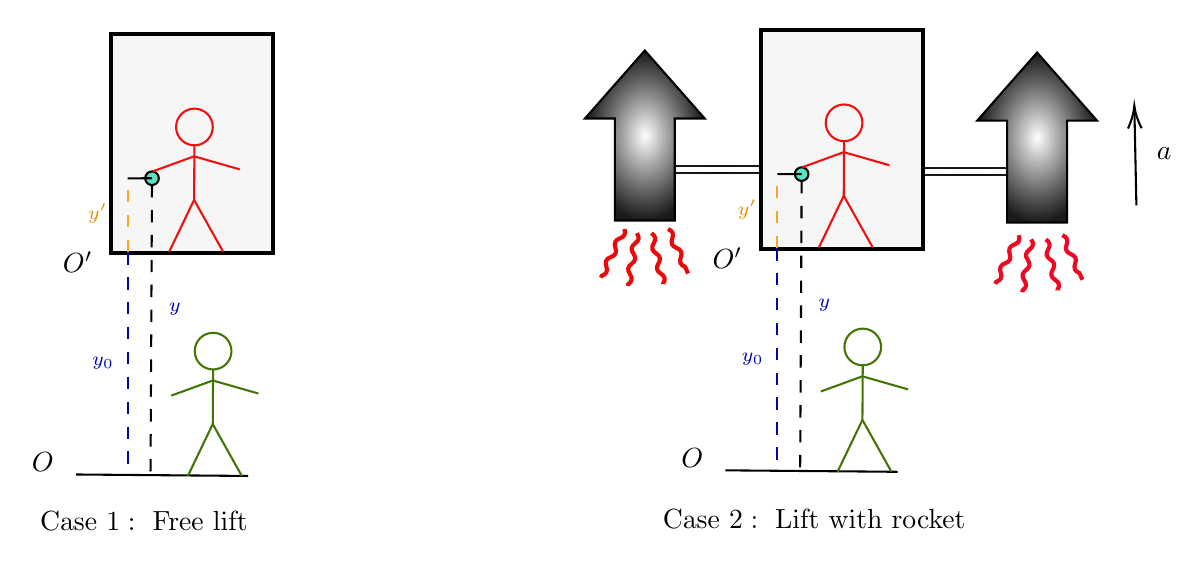
\begin{tikzpicture}[x=0.75pt,y=0.75pt,yscale=-1,xscale=1]
%uncomment if require: \path (0,324); %set diagram left start at 0, and has height of 324

%Shape: Rectangle [id:dp8905660164719159] 
\draw  [fill={rgb, 255:red, 155; green, 155; blue, 155 }  ,fill opacity=0.09 ][line width=1.5]  (103.68,39) -- (181.68,39) -- (181.68,144.62) -- (103.68,144.62) -- cycle ;
%Straight Lines [id:da6981803315105324] 
\draw    (169.68,251.98) -- (86.68,251.27) ;
%Shape: Circle [id:dp17338996810280072] 
\draw  [color={rgb, 255:red, 65; green, 117; blue, 5 }  ,draw opacity=1 ] (144,191.84) .. controls (144,186.96) and (147.96,183) .. (152.84,183) .. controls (157.72,183) and (161.68,186.96) .. (161.68,191.84) .. controls (161.68,196.72) and (157.72,200.68) .. (152.84,200.68) .. controls (147.96,200.68) and (144,196.72) .. (144,191.84) -- cycle ;
%Straight Lines [id:da9228285233233254] 
\draw [color={rgb, 255:red, 65; green, 117; blue, 5 }  ,draw opacity=1 ]   (152.84,200.68) -- (152.68,226.98) ;
%Straight Lines [id:da22779114187554061] 
\draw [color={rgb, 255:red, 65; green, 117; blue, 5 }  ,draw opacity=1 ]   (152.68,226.98) -- (140.68,251.98) ;
%Straight Lines [id:da03636752339232807] 
\draw [color={rgb, 255:red, 65; green, 117; blue, 5 }  ,draw opacity=1 ]   (152.68,226.98) -- (166.68,251.98) ;
%Straight Lines [id:da4065974175639576] 
\draw [color={rgb, 255:red, 65; green, 117; blue, 5 }  ,draw opacity=1 ]   (152.68,205.98) -- (132.68,213.27) ;
%Straight Lines [id:da26319314402387983] 
\draw [color={rgb, 255:red, 65; green, 117; blue, 5 }  ,draw opacity=1 ]   (174.68,212.27) -- (152.68,205.98) ;

%Shape: Circle [id:dp4734164783053887] 
\draw  [fill={rgb, 255:red, 80; green, 227; blue, 194 }  ,fill opacity=0.96 ] (120.13,108.54) .. controls (120.13,106.73) and (121.59,105.27) .. (123.4,105.27) .. controls (125.21,105.27) and (126.68,106.73) .. (126.68,108.54) .. controls (126.68,110.35) and (125.21,111.82) .. (123.4,111.82) .. controls (121.59,111.82) and (120.13,110.35) .. (120.13,108.54) -- cycle ;
%Straight Lines [id:da09568912956647257] 
\draw  [dash pattern={on 4.5pt off 4.5pt}]  (123.4,111.82) -- (122.68,251.82) ;
%Straight Lines [id:da061771502285206115] 
\draw [color={rgb, 255:red, 1; green, 6; blue, 170 }  ,draw opacity=1 ] [dash pattern={on 4.5pt off 4.5pt}]  (111.68,144.18) -- (111.68,252.18) ;
%Straight Lines [id:da28970723992344893] 
\draw [color={rgb, 255:red, 245; green, 166; blue, 35 }  ,draw opacity=1 ] [dash pattern={on 4.5pt off 4.5pt}]  (111.68,144.18) -- (111.68,108.6) ;
%Straight Lines [id:da47063846869304193] 
\draw    (123.4,108.54) -- (111.68,108.6) ;
%Shape: Circle [id:dp3667313637291918] 
\draw  [color={rgb, 255:red, 240; green, 14; blue, 14 }  ,draw opacity=1 ] (135,83.84) .. controls (135,78.96) and (138.96,75) .. (143.84,75) .. controls (148.72,75) and (152.68,78.96) .. (152.68,83.84) .. controls (152.68,88.72) and (148.72,92.68) .. (143.84,92.68) .. controls (138.96,92.68) and (135,88.72) .. (135,83.84) -- cycle ;
%Straight Lines [id:da6276260445486568] 
\draw [color={rgb, 255:red, 240; green, 14; blue, 14 }  ,draw opacity=1 ]   (143.84,92.68) -- (143.68,118.98) ;
%Straight Lines [id:da8718682137405052] 
\draw [color={rgb, 255:red, 240; green, 14; blue, 14 }  ,draw opacity=1 ]   (143.68,118.98) -- (131.68,143.98) ;
%Straight Lines [id:da1353480031793155] 
\draw [color={rgb, 255:red, 240; green, 14; blue, 14 }  ,draw opacity=1 ]   (143.68,118.98) -- (157.68,143.98) ;
%Straight Lines [id:da5690468619727813] 
\draw [color={rgb, 255:red, 240; green, 14; blue, 14 }  ,draw opacity=1 ]   (143.68,97.98) -- (123.68,105.27) ;
%Straight Lines [id:da027974273242843406] 
\draw [color={rgb, 255:red, 240; green, 14; blue, 14 }  ,draw opacity=1 ]   (165.68,104.27) -- (143.68,97.98) ;

%Shape: Rectangle [id:dp5223808571813269] 
\draw  [fill={rgb, 255:red, 155; green, 155; blue, 155 }  ,fill opacity=0.09 ][line width=1.5]  (416.68,37) -- (494.68,37) -- (494.68,142.62) -- (416.68,142.62) -- cycle ;
%Straight Lines [id:da5186712228562469] 
\draw    (482.68,249.98) -- (399.68,249.27) ;
%Shape: Circle [id:dp11607928835249681] 
\draw  [color={rgb, 255:red, 65; green, 117; blue, 5 }  ,draw opacity=1 ] (457,189.84) .. controls (457,184.96) and (460.96,181) .. (465.84,181) .. controls (470.72,181) and (474.68,184.96) .. (474.68,189.84) .. controls (474.68,194.72) and (470.72,198.68) .. (465.84,198.68) .. controls (460.96,198.68) and (457,194.72) .. (457,189.84) -- cycle ;
%Straight Lines [id:da4763789316494623] 
\draw [color={rgb, 255:red, 65; green, 117; blue, 5 }  ,draw opacity=1 ]   (465.84,198.68) -- (465.68,224.98) ;
%Straight Lines [id:da7058069002087343] 
\draw [color={rgb, 255:red, 65; green, 117; blue, 5 }  ,draw opacity=1 ]   (465.68,224.98) -- (453.68,249.98) ;
%Straight Lines [id:da3477827769001153] 
\draw [color={rgb, 255:red, 65; green, 117; blue, 5 }  ,draw opacity=1 ]   (465.68,224.98) -- (479.68,249.98) ;
%Straight Lines [id:da7751166516393394] 
\draw [color={rgb, 255:red, 65; green, 117; blue, 5 }  ,draw opacity=1 ]   (465.68,203.98) -- (445.68,211.27) ;
%Straight Lines [id:da5461672126021012] 
\draw [color={rgb, 255:red, 65; green, 117; blue, 5 }  ,draw opacity=1 ]   (487.68,210.27) -- (465.68,203.98) ;

%Shape: Circle [id:dp5254425366688724] 
\draw  [fill={rgb, 255:red, 80; green, 227; blue, 194 }  ,fill opacity=0.96 ] (433.13,106.54) .. controls (433.13,104.73) and (434.59,103.27) .. (436.4,103.27) .. controls (438.21,103.27) and (439.68,104.73) .. (439.68,106.54) .. controls (439.68,108.35) and (438.21,109.82) .. (436.4,109.82) .. controls (434.59,109.82) and (433.13,108.35) .. (433.13,106.54) -- cycle ;
%Straight Lines [id:da6337699050691787] 
\draw  [dash pattern={on 4.5pt off 4.5pt}]  (436.4,109.82) -- (435.68,249.82) ;
%Straight Lines [id:da3875357225813263] 
\draw [color={rgb, 255:red, 1; green, 6; blue, 170 }  ,draw opacity=1 ] [dash pattern={on 4.5pt off 4.5pt}]  (424.68,142.18) -- (424.68,250.18) ;
%Straight Lines [id:da4326145743966422] 
\draw [color={rgb, 255:red, 245; green, 166; blue, 35 }  ,draw opacity=1 ] [dash pattern={on 4.5pt off 4.5pt}]  (424.68,142.18) -- (424.68,106.6) ;
%Straight Lines [id:da9003426270617577] 
\draw    (436.4,106.54) -- (424.68,106.6) ;
%Shape: Circle [id:dp27147310636592514] 
\draw  [color={rgb, 255:red, 240; green, 14; blue, 14 }  ,draw opacity=1 ] (448,81.84) .. controls (448,76.96) and (451.96,73) .. (456.84,73) .. controls (461.72,73) and (465.68,76.96) .. (465.68,81.84) .. controls (465.68,86.72) and (461.72,90.68) .. (456.84,90.68) .. controls (451.96,90.68) and (448,86.72) .. (448,81.84) -- cycle ;
%Straight Lines [id:da6956644215155984] 
\draw [color={rgb, 255:red, 240; green, 14; blue, 14 }  ,draw opacity=1 ]   (456.84,90.68) -- (456.68,116.98) ;
%Straight Lines [id:da9088074942955296] 
\draw [color={rgb, 255:red, 240; green, 14; blue, 14 }  ,draw opacity=1 ]   (456.68,116.98) -- (444.68,141.98) ;
%Straight Lines [id:da0670900205069288] 
\draw [color={rgb, 255:red, 240; green, 14; blue, 14 }  ,draw opacity=1 ]   (456.68,116.98) -- (470.68,141.98) ;
%Straight Lines [id:da9630372735835703] 
\draw [color={rgb, 255:red, 240; green, 14; blue, 14 }  ,draw opacity=1 ]   (456.68,95.98) -- (436.68,103.27) ;
%Straight Lines [id:da03327171926788586] 
\draw [color={rgb, 255:red, 240; green, 14; blue, 14 }  ,draw opacity=1 ]   (478.68,102.27) -- (456.68,95.98) ;

%Up Arrow [id:dp3302566288814984] 
\path  [shading=_hj4w3dgfv,_w72v0kx56,path fading= _6bmw5izud ,fading transform={xshift=2}] (332,79.76) -- (360.84,47) -- (389.68,79.76) -- (375.26,79.76) -- (375.26,128.9) -- (346.42,128.9) -- (346.42,79.76) -- cycle ; % for fading 
 \draw   (332,79.76) -- (360.84,47) -- (389.68,79.76) -- (375.26,79.76) -- (375.26,128.9) -- (346.42,128.9) -- (346.42,79.76) -- cycle ; % for border 

%Straight Lines [id:da8760871251013267] 
\draw [shading=_kqk1h0g2k,_c8ziououu,path fading= _931hk7ik0 ,fading transform={xshift=2}]   (374.68,102.8) -- (415.68,102.8)(374.68,105.8) -- (415.68,105.8) ;

%Up Arrow [id:dp23881564814673806] 
\path  [shading=_lm7svbvy3,_d447r97wy,path fading= _9nyljxk6y ,fading transform={xshift=2}] (578.68,80.76) -- (549.84,48) -- (521,80.76) -- (535.42,80.76) -- (535.42,129.9) -- (564.26,129.9) -- (564.26,80.76) -- cycle ; % for fading 
 \draw   (578.68,80.76) -- (549.84,48) -- (521,80.76) -- (535.42,80.76) -- (535.42,129.9) -- (564.26,129.9) -- (564.26,80.76) -- cycle ; % for border 

%Straight Lines [id:da08896072146414558] 
\draw [shading=_9xm9bjwtq,_g2k2mc5so,path fading= _t429ztxrk ,fading transform={xshift=2}]   (536,106.8) -- (495,106.8)(536,103.8) -- (495,103.8) ;

%Straight Lines [id:da9252657014634662] 
\draw [color={rgb, 255:red, 235; green, 9; blue, 9 }  ,draw opacity=1 ][line width=1.5]    (351,133) .. controls (351.78,135.23) and (351.06,136.73) .. (348.83,137.5) .. controls (346.6,138.28) and (345.88,139.78) .. (346.65,142.01) .. controls (347.43,144.24) and (346.71,145.74) .. (344.48,146.51) .. controls (342.25,147.28) and (341.53,148.78) .. (342.31,151.01) .. controls (343.08,153.24) and (342.36,154.74) .. (340.13,155.52) -- (339.68,156.45) -- (339.68,156.45) ;
%Straight Lines [id:da449504739304021] 
\draw [color={rgb, 255:red, 235; green, 9; blue, 9 }  ,draw opacity=1 ][line width=1.5]    (372,133) .. controls (374.21,133.83) and (374.89,135.35) .. (374.06,137.56) .. controls (373.23,139.76) and (373.91,141.28) .. (376.11,142.11) .. controls (378.32,142.94) and (379,144.46) .. (378.17,146.67) .. controls (377.34,148.88) and (378.02,150.4) .. (380.23,151.23) -- (381.68,154.45) -- (381.68,154.45) ;
%Straight Lines [id:da29049965893706386] 
\draw [color={rgb, 255:red, 235; green, 9; blue, 9 }  ,draw opacity=1 ][line width=1.5]    (357,135) .. controls (358.36,136.92) and (358.08,138.56) .. (356.16,139.93) .. controls (354.24,141.3) and (353.96,142.94) .. (355.33,144.86) .. controls (356.69,146.78) and (356.41,148.42) .. (354.49,149.79) .. controls (352.57,151.16) and (352.29,152.8) .. (353.66,154.72) .. controls (355.02,156.64) and (354.74,158.28) .. (352.82,159.65) -- (352.68,160.45) -- (352.68,160.45) ;
%Straight Lines [id:da8972864374449925] 
\draw [color={rgb, 255:red, 235; green, 9; blue, 9 }  ,draw opacity=1 ][line width=1.5]    (364,135) .. controls (366,136.25) and (366.38,137.87) .. (365.13,139.87) .. controls (363.88,141.87) and (364.26,143.49) .. (366.26,144.74) .. controls (368.26,145.99) and (368.64,147.61) .. (367.4,149.61) .. controls (366.15,151.61) and (366.53,153.23) .. (368.53,154.48) .. controls (370.53,155.73) and (370.91,157.35) .. (369.66,159.35) -- (369.68,159.45) -- (369.68,159.45) ;
%Straight Lines [id:da8506836264898309] 
\draw [color={rgb, 255:red, 237; green, 9; blue, 36 }  ,draw opacity=1 ][line width=1.5]    (541,136) .. controls (541.78,138.23) and (541.06,139.73) .. (538.83,140.5) .. controls (536.6,141.28) and (535.88,142.78) .. (536.65,145.01) .. controls (537.43,147.24) and (536.71,148.74) .. (534.48,149.51) .. controls (532.25,150.28) and (531.53,151.78) .. (532.31,154.01) .. controls (533.08,156.24) and (532.36,157.74) .. (530.13,158.52) -- (529.68,159.45) -- (529.68,159.45) ;
%Straight Lines [id:da149084529134893] 
\draw [color={rgb, 255:red, 237; green, 9; blue, 36 }  ,draw opacity=1 ][line width=1.5]    (562,136) .. controls (564.21,136.83) and (564.89,138.35) .. (564.06,140.56) .. controls (563.23,142.76) and (563.91,144.28) .. (566.11,145.11) .. controls (568.32,145.94) and (569,147.46) .. (568.17,149.67) .. controls (567.34,151.88) and (568.02,153.4) .. (570.23,154.23) -- (571.68,157.45) -- (571.68,157.45) ;
%Straight Lines [id:da7907638543224793] 
\draw [color={rgb, 255:red, 237; green, 9; blue, 36 }  ,draw opacity=1 ][line width=1.5]    (547,138) .. controls (548.36,139.92) and (548.08,141.56) .. (546.16,142.93) .. controls (544.24,144.3) and (543.96,145.94) .. (545.33,147.86) .. controls (546.69,149.78) and (546.41,151.42) .. (544.49,152.79) .. controls (542.57,154.16) and (542.29,155.8) .. (543.66,157.72) .. controls (545.02,159.64) and (544.74,161.28) .. (542.82,162.65) -- (542.68,163.45) -- (542.68,163.45) ;
%Straight Lines [id:da3525417892092241] 
\draw [color={rgb, 255:red, 237; green, 9; blue, 36 }  ,draw opacity=1 ][line width=1.5]    (554,138) .. controls (556,139.25) and (556.38,140.87) .. (555.13,142.87) .. controls (553.88,144.87) and (554.26,146.49) .. (556.26,147.74) .. controls (558.26,148.99) and (558.64,150.61) .. (557.4,152.61) .. controls (556.15,154.61) and (556.53,156.23) .. (558.53,157.48) .. controls (560.53,158.73) and (560.91,160.35) .. (559.66,162.35) -- (559.68,162.45) -- (559.68,162.45) ;
%Straight Lines [id:da28805676008620384] 
\draw    (597.68,121.65) -- (596.72,75.6) ;
\draw [shift={(596.68,73.6)}, rotate = 88.81] [color={rgb, 255:red, 0; green, 0; blue, 0 }  ][line width=0.75]    (10.93,-3.29) .. controls (6.95,-1.4) and (3.31,-0.3) .. (0,0) .. controls (3.31,0.3) and (6.95,1.4) .. (10.93,3.29)   ;

% Text Node
\draw (93,193.4) node [anchor=north west][inner sep=0.75pt]  [font=\scriptsize,color={rgb, 255:red, 1; green, 6; blue, 170 }  ,opacity=1 ]  {$y_{0}$};
% Text Node
\draw (130,167.4) node [anchor=north west][inner sep=0.75pt]  [font=\scriptsize,color={rgb, 255:red, 1; green, 6; blue, 170 }  ,opacity=1 ]  {$y$};
% Text Node
\draw (91,119.4) node [anchor=north west][inner sep=0.75pt]  [font=\scriptsize,color={rgb, 255:red, 230; green, 139; blue, 8 }  ,opacity=1 ]  {$y'$};
% Text Node
\draw (64,239.4) node [anchor=north west][inner sep=0.75pt]    {$O$};
% Text Node
\draw (79,142.4) node [anchor=north west][inner sep=0.75pt]    {$O'$};
% Text Node
\draw (406,191.4) node [anchor=north west][inner sep=0.75pt]  [font=\scriptsize,color={rgb, 255:red, 1; green, 6; blue, 170 }  ,opacity=1 ]  {$y_{0}$};
% Text Node
\draw (443,165.4) node [anchor=north west][inner sep=0.75pt]  [font=\scriptsize,color={rgb, 255:red, 1; green, 6; blue, 170 }  ,opacity=1 ]  {$y$};
% Text Node
\draw (404,117.4) node [anchor=north west][inner sep=0.75pt]  [font=\scriptsize,color={rgb, 255:red, 230; green, 139; blue, 8 }  ,opacity=1 ]  {$y'$};
% Text Node
\draw (377,237.4) node [anchor=north west][inner sep=0.75pt]    {$O$};
% Text Node
\draw (392,140.4) node [anchor=north west][inner sep=0.75pt]    {$O'$};
% Text Node
\draw (68,267.4) node [anchor=north west][inner sep=0.75pt]    {$\mathrm{Case\ 1:\ Free\ lift}$};
% Text Node
\draw (368,266.4) node [anchor=north west][inner sep=0.75pt]    {$\mathrm{Case\ 2:\ Lift\ with\ rocket}$};
% Text Node
\draw (606,92.4) node [anchor=north west][inner sep=0.75pt]    {$a$};


\end{tikzpicture}
